\chapter{Completion in Pharo}
\label{chap:PharoCompletion}

In this chapter, I give a detailed overview of the current completion engine in the Pharo IDE, as well as describe the challenges of code completion for a dynamically typed language, and the idea behind the sorter plugin.

\section{Code Completion Background}
\label{sec:PharoCompletion-Background}
The Pharo programming language is an object-oriented dynamically typed programming language which is inspired by Smalltalk. The Pharo IDE is a programming environment meant specifically for developing in Pharo. It consists of a virtual machine (VM), on top of which an image, serving as the current IDE workspace, can be run.

The Pharo IDE itself is written in Pharo and can be extended from within. This means that when implementing code completion, one can test it live in the very environment where one is developing it, which, if not done carefully, can lead to breaking the system.

Code completion in the Pharo IDE is called at every keystroke, as soon as two and more alphabetic characters are typed in. A completion context gets created for the text typed in until then, regardless of the type of the code editor. And there are several code editor tools within the Pharo IDE, such as:
\begin{itemize}
    \item the Playground, which is a tool for generating small scripts and sketching out some code
    \item the System Browser, a tool which allows one to browse classes and methods and has a dedicated code area for writing and editing code
    \item the Debugger, a specialised code editor for editing code during debugging
\end{itemize}
(Figures \ref{fig:playground} and \ref{fig:editor} demonstrate the way the completion menu looks in the Playground and the System Browser).

\section{Typing for Completion in Dynamic Languages}
\label{sec:PharoCompletion-Typing}
As Pharo is a dynamically typed language, the precise type information is only available at runtime. Not knowing the type when typing can make the completion suggestions less precise and push relevant options to the bottom of the list of completions, which then requires scrolling or typing more characters.

\begin{figure}[H]
    \centering
    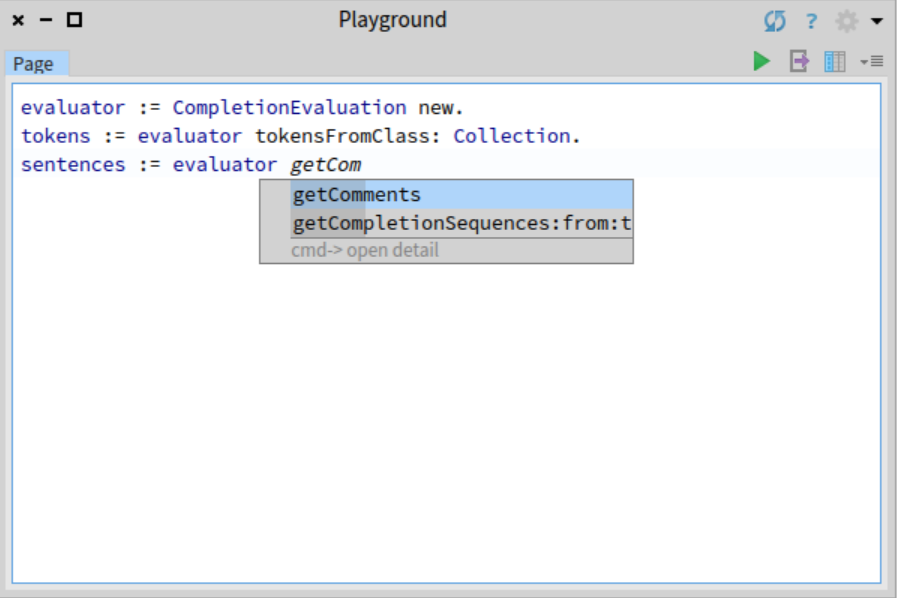
\includegraphics[width=0.9\linewidth]{images/completion1.png}
    \caption{Completion in the Playground}
    \label{fig:playground}
\end{figure}

\begin{figure}[H]
    \centering
    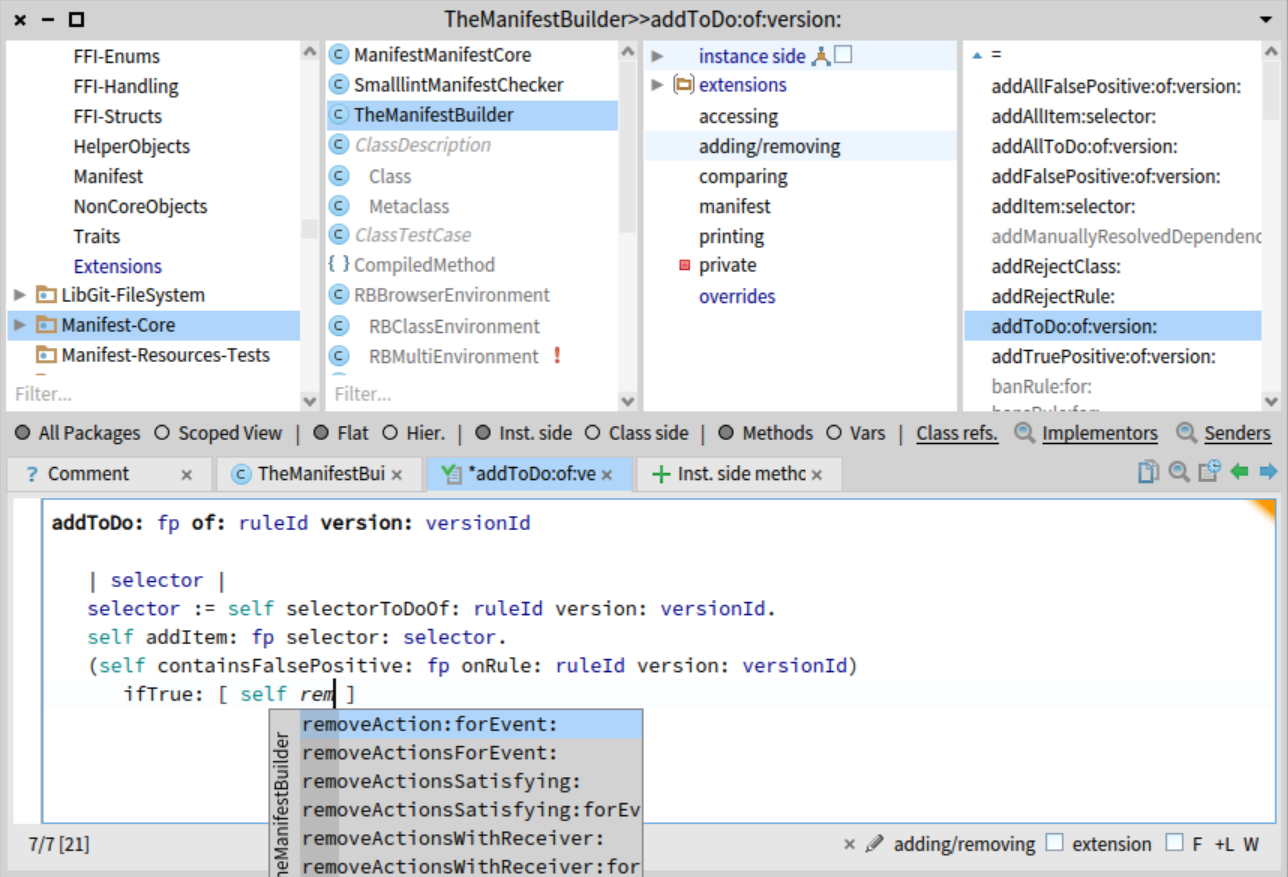
\includegraphics[width=0.9\linewidth]{images/completion2.png}
    \caption{Completion in the System Browser}
    \label{fig:editor}
\end{figure}

There are a couple of approaches one could take to solve this. The first is type \footnote{\textit{Type} meaning a kind of variable, instead of an act of writing something by pressing the keys. Throughout this text the word is often used in either one of meaning, depending on the context.} inference (or rather type reconstruction), which can be done by extracting type information by looking at the messages sent to a variable, and merging these results with types found by heuristics applied to the right-hand side of assignment expressions (\cite{Pluq09a}). Type guessing by means of name analysis can also be done, but it is more likely to be misleading. The third approach involves the AST-based completion in the Pharo IDE (more details in the next section). It performs a semantic analysis of source code, which provides us with more accurate type information for certain kinds of nodes.

\section{AST-Based Completion}
\label{sec:PharoCompletion-ASTCompletion}
The completion context parses the text and transforms it into the AST representation, such as a sequence of AST nodes. In the process, all the information needed for further actions is extracted: the current position of the cursor (where we want to get the completion) and the class which we are currently modifying (or information that the completion happens in the Playground, for which there is no such data). By performing the semantic analysis, we get the most suitable type of node for each part of code, and then visit each node to get the correct completion behaviour (i.e. contextually appropriate suggestions). For instance, this means that for a Global node, we want to suggest all the globals, such as class names, for a Message node we only want to get message sends to a variable, and so on.

Combining the available prefix of length at least 2, as well as relevant semantic information, we give a list of suitable completion suggestions that are then passed to the sorter. The list itself is displayed in a completion menu that pops up once the completion is called and then is updated with every new keystroke, unless the developer \footnote{Developer in the Pharo IDE who is a user of code completion} cancels it by pressing \textit{Esc} or clicking outside of the text area. The completion window can also disappear once there are no valid suggestions to give anymore.

\section{Sorter Plugin}
\label{sec:PharoCompletion-SorterPlugin}
The sorter plugin is an important part of the code completion tool in the Pharo IDE which is responsible for the final order in which the completions are presented. Within the sorter, we treat the completion implementation as a black box. The only information it receives is the list of completions to be sorted and the context (meaning any other completion-related information, such as the AST node, the cursor position, the class where the completion happens (if known), and so on). This was done to make the sorter extendable and open for modification, so one could take the general completion functionality and then on top of it put any sorting strategy they would like to have.

This means that the way we get the completion results is the same every time (i.e. we get contextually suitable completions as a result of analysing the AST). However, the sorting strategy vastly influences the end result (i.e. the list of suggestions displayed in the pop-up completion menu) the users (developers) see. Specifically, a good sorter can prioritise the more relevant results that can be positioned far down the list of suggestions (for example, if the type of the token being completed is not known or there is no local context, as in the Playground).

\section{Summary}
\label{sec:PharoCompletion-Summary}
\begin{itemize}
    \item Pharo is an object-oriented dynamically typed language inspired by Smalltalk, and the Pharo IDE is a programming environment intended for developing in Pharo.
    \item Code completion in the Pharo IDE is used in the code editors, the list of which included the Playground (a scripting tool), the System Browser (a tool for browsing, writing and editing class functionality), et cetera.
    \item Current code completion is based on analysing the AST of source code; it is called after the developer types two alphabetic characters, and the completion candidates are suggested by the most relevant semantic context.
    \item Other than the completion engine, responsible for the process of \textit{completing} code, another important part of the code completion tool is the sorter plugin that supports implementing various sorting strategies. It is responsible for the order in which the results are displayed to the user.
\end{itemize}